\documentclass[crop,tikz,convert={outext=.svg,command=\unexpanded{pdf2svg \infile\space\outfile}},multi=false]{standalone}[2012/04/13]
\usepackage{tikz}
\usepackage{pgfplots}
\usepackage{tikz}
\usetikzlibrary{calc}
\tikzset{stretch/.initial=1}
\newcommand\drawloop[4][]%
{\draw[shorten <=0pt, shorten >=0pt,#1]
	($(#2)!\pgfkeysvalueof{/tikz/stretch}!(#2.#3)$)
	let \p1=($(#2.center)!\pgfkeysvalueof{/tikz/stretch}!(#2.north)-(#2)$),
	\n1= {veclen(\x1,\y1)*sin(0.5*(#4-#3))/sin(0.5*(180-#4+#3))}
	in arc [start angle={#3-90}, end angle={#4+90}, radius=\n1]%
}
\usetikzlibrary{arrows,shapes,positioning}
\begin{document}
	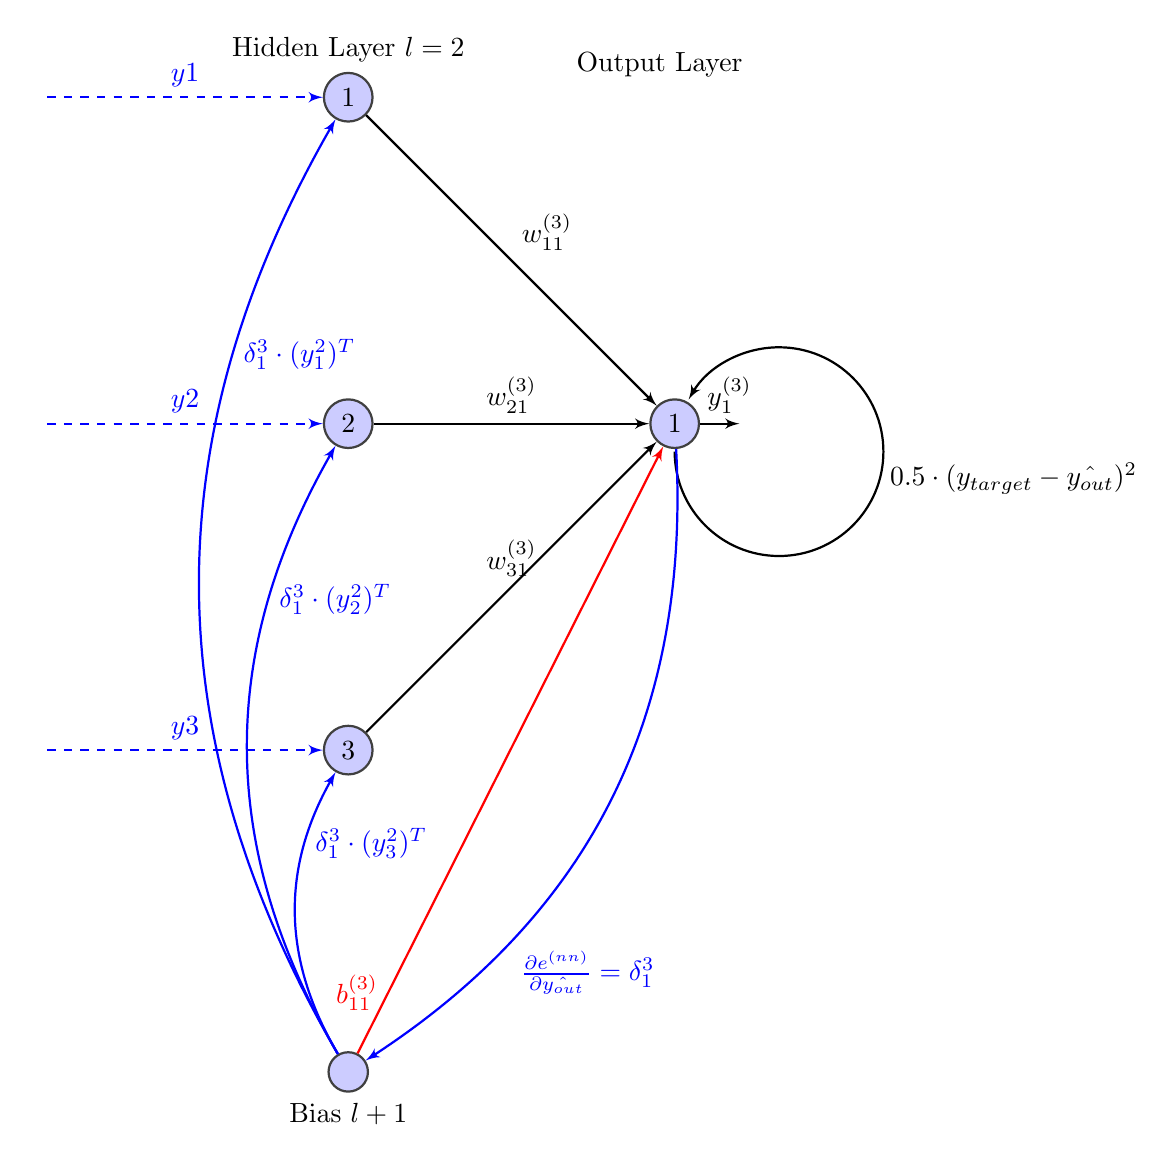
\begin{tikzpicture}[->,>=latex',shorten >=0pt,auto,node distance=3.5cm,
		thick]
		\tikzstyle{komp}=[rectangle,thick,draw=black!75,fill=black!0,minimum size=10mm]
		\tikzstyle{sum_punkt}=[circle,thick,draw=black!75,fill=black!0,minimum size=3mm]
		\tikzstyle{black_point}=[circle,thick,inner sep=0pt,draw=black!75,fill=black!100,minimum size=1mm]
		\tikzstyle{get}=[circle,thick,draw=black!75,fill=black!0,minimum size=5mm]
		\tikzstyle{agt}=[rectangle,thick,draw=black!75,fill=blue!25,minimum size=10mm]
		\tikzstyle{komp2}=[rectangle,thick,draw=black,minimum size=10mm]
		\tikzstyle{mot2}=[circle,thick,draw=black!75,fill=blue!20,minimum size=5mm]
		
		\node[] (black_point_vor_regler) {};
		\node[] (black_point_vor_regler1) [below=of black_point_vor_regler] {};
		\node[] (black_point_vor_regler2) [below=of black_point_vor_regler1] {};
		
		\node[mot2, align=center,label={Hidden Layer $l=2$}] (hidden11) [right=of black_point_vor_regler] {1};
		\node[mot2, align=center] (hidden12)[below=of hidden11] {2};
		\node[mot2, align=center] (hidden13)[below=of hidden12] {3};
			
		\node[mot2, align=center] (output)[right=of hidden12] {1};
		\node[] (ghostoutput) [right=0.5cm of output] {};
		
		\node[label={Output Layer}] (label_output) [right= of hidden11]{};
		\node[mot2,align=center,label=below:{Bias $l+1$}] (bias3) [below=of hidden13] {};
		\draw[red,->](bias3)--node[pos=0.1,left] {$b^{(3)}_{11}$}(output);
		\draw[->](hidden11)--node[pos=0.5,above right] {$w^{(3)}_{11}$}(output);
		\draw[->](hidden12)--node[pos=0.5,above] {$w^{(3)}_{21}$}(output);
		\draw[->](hidden13)--node[pos=0.5,above] {$w^{(3)}_{31}$}(output);
		\draw[->] (output) -- node[near end] {$y^{(3)}_1$} (ghostoutput);
		\drawloop[->,stretch=1.1]{output}{270}{420} node[pos=0.5,right]{$0.5 \cdot (y_{target}-\hat{y_{out}})^2$};
		\draw[blue,->,bend left] (output)  to node[near end] {$\frac{\partial e^{(nn)}}{\partial\hat{y_{out}}} = \delta_{1}^{3}$}(bias3);
		\draw[blue,->,bend left] (bias3)  to node[right,near end] {$\delta_{1}^{3} \cdot (y_1^{2})^{T}$}(hidden11);
		\draw[blue,->,bend left] (bias3)  to node[right,near end] {$\delta_{1}^{3} \cdot (y_2^{2})^{T}$}(hidden12);
		\draw[blue,->,bend left] (bias3)  to node[right,near end] {$\delta_{1}^{3} \cdot (y_3^{2})^{T}$}(hidden13);
		\node[] (hl1) [left=3.5cm of hidden11] {};
		\node[] (hl2) [left=3.5cm of hidden12] {};
		\node[] (hl3) [left=3.5cm of hidden13] {};
		\draw[blue,dashed,->](hl1) to node {$y1$}(hidden11);
		\draw[blue,dashed,->](hl2) to node {$y2$}(hidden12);
		\draw[blue,dashed,->](hl3) to node {$y3$}(hidden13);
		%\draw[red,thick,<->] (output.-90) arc (180:180+264:4);
	\end{tikzpicture}
\end{document}